%%%
%
% $Autor: Wings $
% $Datum: 2021-05-14 $
% $Pfad: LEDRGBExternal $
% $Dateiname: 
% $Version: 4620 $
%
% !TeX spellcheck = de_DE/GB
% !TeX program = pdflatex
% !BIB program = biber/bibtex
% !TeX encoding = utf8
%
%%%

%todo citations
%todo create tikz pictures
%todo create sketches /ino-files with the code
%todo test the code


% Farben: https://rgbcolorcode.com/color/00FF00

\chapter{External RGB-LED}


\section{Standard RGB-LED}\index{LED!Standard RGB-LED}

An RGB-LED is a type of \ac{led} that can emit different colors of light. RGB stands for red, green, and blue, which are the three primary colors of light. An RGB-LED consists of three individual \ac{led}s inside a single package, each with its own color and pin. By varying the brightness of each \ac{led} using \ac{pwm} signals, an RGB-LED can produce a wide range of colors by mixing the primary colors. An RGB-LED is usually active-low, which means that setting the pin to LOW will turn the \ac{led} on, and setting the pin to HIGH will turn the \ac{led} off. 


To connect a RGB-LED to an Arduino Nano 33 BLE Sense board, you need to use three resistors, one for each color pin. The value of the resistors depends on the type and specifications of the RGB \ac{led}, but a common value is 220 ohms. You also need to connect the common cathode or anode of the RGB-LED to the ground or 3.3V pin of the board, respectively. Here is a diagram that shows how to connect a common cathode RGB \ac{led} to the board:


\Mynote{create  a diagram that shows how to connect a common cathode RGB-LED to the board}




\begin{center}
    %todo tikz picture with strip red - red - black - brown 1\%
    % or red - red - black - gold 5\%
    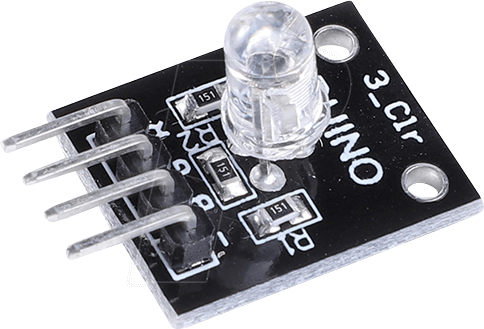
\includegraphics[width=0.8\textwidth]{Sensor/LED/RGB}
    \captionof{figure}{External RGB-LED with Resistors \cite{Simac:2020}}
\end{center}


External RGB-LED with Resistors \cite{Simac:2020,Kingbright:2010}



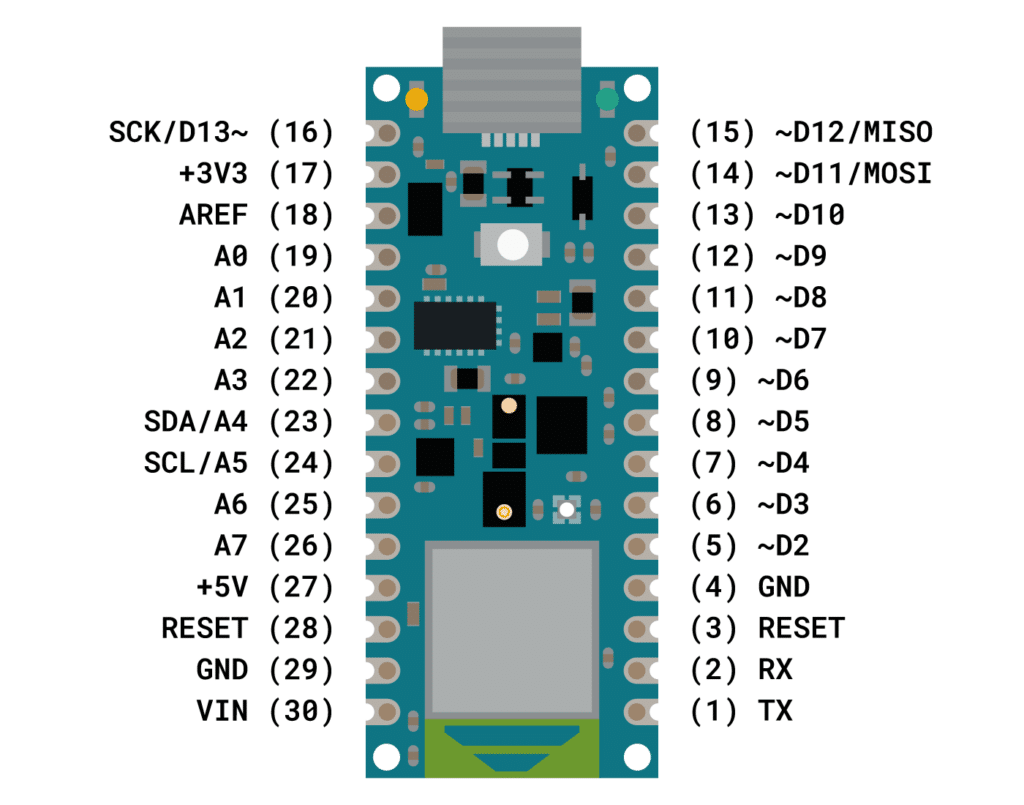
\includegraphics[width=0.8\textwidth]{Arduino/Nano33BLE/arduino-nano-33-ble-sense-pinout-1024x805.png}


\begin{center}
  %todo tikz picture on RGB-LED 
  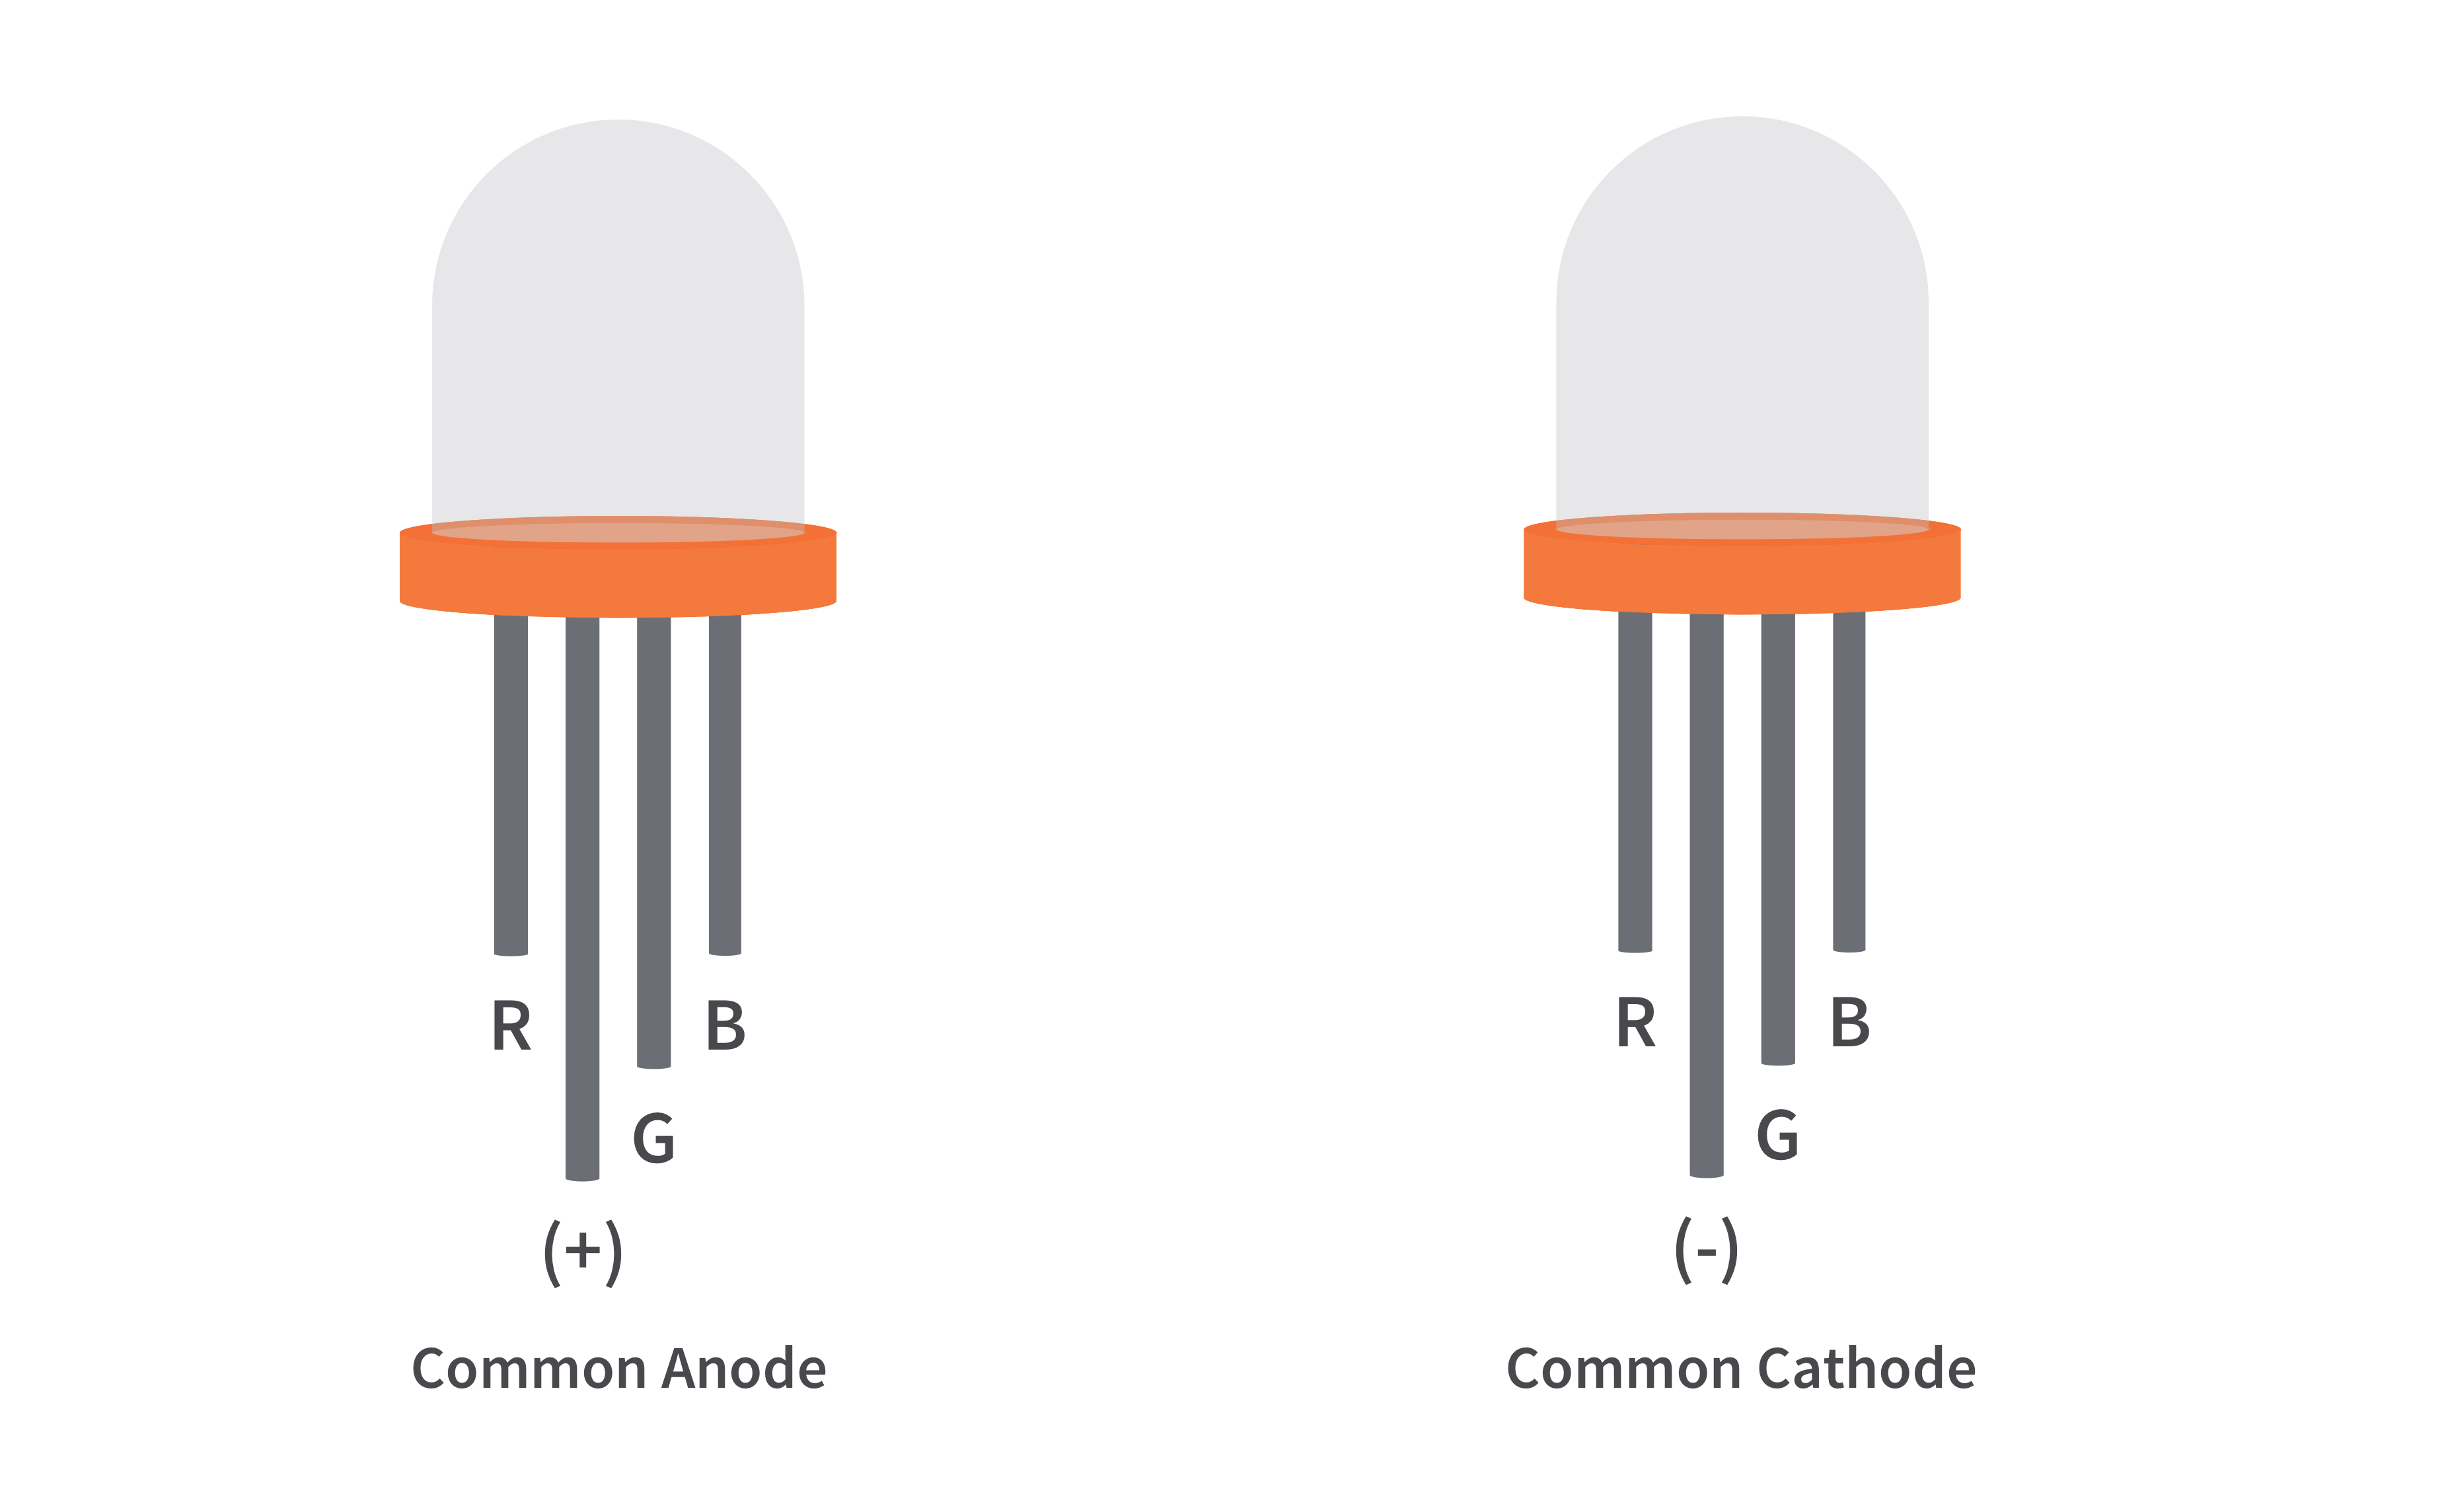
\includegraphics[width=0.8\textwidth]{Sensor/LED/RGB-LEDs-Pinout.png}
  \captionof{figure}{Connectors of a RGB-LED.}
\end{center}


\section{Specific Sensor}

\Mynote{take a LED or RGB-LED}

\Mynote{citation}




\subsection{Pins}

Here, you can define some pins for \ac{led}s. 

\Mynote{Which one}

This must be observed when using the pins.



\begin{description}
    \item [Red LED:] LEDR = Pin 22
    \item [Green LED:] LEDG = Pin 23
    \item [Blue LED:] LEDB = Pin 24
\end{description}



\section{Specification}

cite data sheet


\section{Calibration}

cite method

\section{Simple Code}


\section{Simple Application}

\section{Tests}

\subsection{Simple Function Test}


To turn ON the \ac{led}s, write a state \PYTHON{HIGH} to the \ac{led}:



\medskip

{
    \begin{Arduino}
        digitalWrite(LEDR, HIGH); //RED
        digitalWrite(LEDG, HIGH); //GREEN
        digitalWrite(LEDB, HIGH); //BLUE
    \end{Arduino}
    \captionof{code}{Swichting On the LEDs}
}

\medskip

To turn OFF the \ac{led}s, write a state \PYTHON{LOW} to the \ac{led}:

\medskip

{
    \begin{Arduino}
        digitalWrite(LEDR, LOW); //RED
        digitalWrite(LEDG, LOW); //GREEN
        digitalWrite(LEDB, LOW); //BLUE
    \end{Arduino}
    \captionof{code}{Swichting Off the LEDs}
}

\bigskip


\subsection{Test all Functions}


\subsection{Brightness of the RGB-LED}\index{LED!Brightness}

In a short cut, using values between 255 - 0 to write to the RGB-LED is possible, too. Then the brightness is defined.

\medskip

{
    \begin{Arduino}
        analogWrite(LEDR, 72);  //GREEN 
        analogWrite(LEDG, 122); //BLUE 
        analogWrite(LEDB, 234); //RED
    \end{Arduino}
    \captionof{code}{value between 255 - 0 to write to the RGB-LED}
}

\bigskip

This sketch \ref{ArduinoLEDBrightness} will make the RGB-LED change colors smoothly by varying the brightness of each \ac{led} with different speeds. You can adjust the initial brightness values and the increment/decrement values to get different effects.

{
    \begin{Arduino}
// Define the pins for the RGB-LED
#define RED_PIN 22
#define GREEN_PIN 23
#define BLUE_PIN 24
        
// Define the initial brightness values for each color (0-255)
int redBrightness = 0;
int greenBrightness = 0;
int blueBrightness = 0;
        
// Define the increment/decrement value for each color
int redStep = 5;
int greenStep = 3;
int blueStep = 7;
        
void setup() {
    // Set the LED pins as outputs
    pinMode(RED_PIN, OUTPUT);
    pinMode(GREEN_PIN, OUTPUT);
    pinMode(BLUE_PIN, OUTPUT);
}
        
void loop() {
    // Write the PWM values to the LED pins
    analogWrite(RED_PIN, redBrightness);
    analogWrite(GREEN_PIN, greenBrightness);
    analogWrite(BLUE_PIN, blueBrightness);
            
    // Update the brightness values for each color
    redBrightness += redStep;
    greenBrightness += greenStep;
    blueBrightness += blueStep;
            
    // Check if the brightness values are out of range and reverse the direction
    if (redBrightness <= 0 || redBrightness >= 255) {
        redStep = -redStep;
    }
    if (greenBrightness <= 0 || greenBrightness >= 255) {
        greenStep = -greenStep;
    }
    if (blueBrightness <= 0 || blueBrightness >= 255) {
        blueStep = -blueStep;
    }
                    
    // Wait for 10 milliseconds
    delay(10);
}
  \end{Arduino}
  \captionof{code}{Different brightness levels for the RGB-LED colors}\label{ArduinoLEDBrightness}
}
        
  \bigskip
        
        
\subsubsection{Colors}\index{LED!Colors}
        
        A RGB-LED is a device that can emit light of different colors by mixing the primary colors of red, green, and blue. The color of the light depends on the relative brightness of each \ac{led}, which can be controlled by \ac{pwm} signals. By varying the brightness of each \ac{led}, the RGB-LED can produce a wide range of colors, such as yellow, cyan, magenta, white, and more. Some examples of the colors and their corresponding brightness values are:
        
        \begin{description}
            \item [Red:] red = 255, green = 0, blue = 0
            \item [Green:] red = 0, green = 255, blue = 0
            \item [Blue:] red = 0, green = 0, blue = 255
            \item [Yellow:] red = 255, green = 255, blue = 0
            \item [Cyan:] red = 0, green = 255, blue = 255
            \item [Magenta:] red = 255, green = 0, blue = 255
            \item [White:] red = 255, green = 255, blue = 255
            \item [Black:] red = 0, green = 0, blue = 0
        \end{description}
        
        \medskip
        
        The RGB-LED can also create intermediate colors by using different brightness values for each \ac{led}. For example, to create
        
        \begin{itemize}
            \item \textbf{orange}, one can use red = 255, green = 127, blue = 0. 
            \item To create \textbf{pink}, one can use red = 255, green = 192, blue = 203. 
            \item To create \textbf{purple}, one can use red = 128, green = 0, blue = 128. 
        \end{itemize}
        
        \medskip
        
        The RGB-LED can also create gradients of colors by changing the brightness values gradually over time. This can create a smooth transition from one color to another, such as from red to green to blue and back to red.


\section{Simple Application}


\section{Further Readings}


